\documentclass[a4paper]{jsarticle}
\usepackage[dvipdfmx]{graphicx}
\usepackage{amsmath}
\usepackage{bm}
\renewcommand{\thesection}{第\arabic{section}問}
\renewcommand{\thesubsection}{(\arabic{subsection})}
\renewcommand{\thesubsubsection}{(\alph{subsubsection})}
\begin{document}

\title{2020分野3}
\author{nakao}
\maketitle

\section{}
\subsection{}
\subsubsection{}
断面流速を$v$とすると、
\begin{equation}
  v = \frac{Q}{A} = \frac{Q}{a h^{\frac{3}{2}}}
\end{equation}
であるから、比エネルギー$E$は、
\begin{equation}
  E = \frac{v^2}{2g} + h = \frac{Q^2}{2g a^2 h^3} + h
\end{equation}
となる。

\subsubsection{}
式(2)を$h$で微分して、
\begin{equation}
  \frac{\partial E}{\partial h} = -\frac{3 Q^2}{2g a^2 h^4} + 1
\end{equation}
を得る。$h = h_c$において$\frac{\partial E}{\partial h} = 0$であるから、
\begin{equation}
  h_c = \left(\frac{3 Q^2}{2 g a^2}\right)^{\frac{1}{4}}
\end{equation}
となる。

\subsubsection{}
式(2),(4)より、
\begin{equation}
  E = \frac{1}{3} h_c^4 h^{-3} + h
\end{equation}
と表される。$h = h_c$をこれに代入して、
\begin{equation}
  E_c = \frac{1}{3} h_c^4 h_c^{-3} + h_c = \frac{4}{3} h_c
\end{equation}
となる。

\subsection{}
開水路の勾配を$I$、開水路断面の径心を$R$、断面流速を$v$とする。\par
ここではManningの式$v = \frac{1}{n} R^{\frac{2}{3}}  I^{\frac{1}{2}}$により摩擦を評価する。
$R = A/s$($s$は潤辺)を用いると、流量$Q$について、
\begin{equation}
  Q = A v = A \frac{1}{n} \left(\frac{A}{s}\right)^{\frac{2}{3}} I^{\frac{1}{2}}
  = \frac{1}{n} A^{\frac{5}{3}} I^{\frac{1}{2}} s^{-\frac{2}{3}}
\end{equation}
を得る。したがって、$Q$を最大化するには$s$を最小化すればよい。
$A$と$h$の間には$A = mh^2$、つまり$h = \sqrt{A/m}$が成り立つことを用いれば、
\begin{equation}
  s = 2 \sqrt{m^2 + 1} h = 2 \sqrt{A \left(m + \frac{1}{m}\right)}
\end{equation}
である。ここで、
\begin{equation}
  f(m) = m + \frac{1}{m}
\end{equation}
とおいて、これを最小化する。
\begin{equation}
  f^{\prime}(m) = 1 - \frac{1}{m^2}
\end{equation}
であり、これを0とすることにより、最適な$m$は$m = 1$である。

\subsection{}
\subsubsection{}
断面流速を$v$とする。
水路の摩擦が無視できるとき、エネルギー保存則
\begin{equation}
  \frac{\mathrm{d}}{\mathrm{d} x} \left(\frac{v^2}{2g} + h + z\right) = 0
\end{equation}
が成り立つ。これと$v = q/h$であることを用いると、
\begin{equation}
  \frac{\mathrm{d} z}{\mathrm{d} x}
  = -\frac{\mathrm{d}}{\mathrm{d} x} \left(\frac{q^2}{2g h^2} + h\right)
  = -\left(-\frac{q^2}{gh^3} + 1\right) \frac{\mathrm{d} h}{\mathrm{d} x}
  = \left(\mathrm{Fr}^2 - 1\right) \frac{\mathrm{d} h}{\mathrm{d} x}
\end{equation}
が得られる。よって、
\begin{equation}
  \frac{\mathrm{d} h}{\mathrm{d} x} = \frac{1}{\mathrm{Fr}^2 - 1} \frac{\mathrm{d} z}{\mathrm{d} x}
\end{equation}
が成り立つ。したがって、
\begin{equation}
  \frac{\mathrm{d} H}{\mathrm{d} x} = \frac{\mathrm{d}}{\mathrm{d} x} (h + z)
  = \left(\frac{1}{\mathrm{Fr}^2 - 1} + 1\right) \frac{\mathrm{d} z}{\mathrm{d} x}
  = \frac{\mathrm{Fr}^2}{\mathrm{Fr}^2 - 1} \frac{\mathrm{d} z}{\mathrm{d} x}
\end{equation}
となる。

\subsubsection{}
常流を仮定すると、$\mathrm{Fr} < 1$である。式(14)より、$z$と$H$の増減は逆になる。
上流側からマウンドのある区間にさしかかると、$z$が増加し$H$が減少し、マウンド頂部を越えると$z$が減少し$H$が増加する。
エネルギー保存則より、マウンドの下流側では$H = h_0$であり、マウンドのある区間では水位が下がっていることになる。

\subsubsection{}
条件を満たすとき、エネルギー保存則より
\begin{equation}
  \frac{q^2}{2g h_c^2} + h_c + z_0 = \frac{q^2}{2g h_0^2} + h_0
\end{equation}
であり、
\begin{equation}
  z_0 = \frac{q^2}{2g} \left(\frac{1}{h_0^2} - \frac{1}{h_c^2}\right) + h_0 - h_c
\end{equation}
となる。

\subsection{}
\subsubsection{}
運動量保存則により、
\begin{equation}
  \rho Q v_1 - \rho Q v_2 = \frac{1}{2} \rho g B_1 h_1^2 - \frac{1}{2} \rho g B_2 h_2^2
\end{equation}
が成り立つ。連続式$Q = B_1 h_1 v_1 = B_2 h_2 v_2$より、
\begin{equation}
  \rho B_1 h_1 v_1^2 - \rho B_2 h_2 v_2^2 = \frac{1}{2} \rho g B_1 h_1^2 - \frac{1}{2} \rho g B_2 h_2^2
\end{equation}
となる。

\subsubsection{}
連続式$B_1 h_1 v_1 = B_2 h_2 v_2$より、
\begin{equation}
  v_2 = \frac{B_1 h_1}{B_2 h_2} v_1 = \frac{1}{A C} v_1
\end{equation}
である。これと$h_2 = A h_1, B_2 = C B_1$を式(18)に代入して、
\begin{equation}
  \rho B_1 h_1 v_1^2 \left(1 - \frac{1}{A C}\right)
  = \frac{1}{2} \rho g B_1 h_1^2 (1 - A^2 C)
\end{equation}
を得る。これより、
\begin{equation}
  \frac{v_1^2}{g h_1} = \frac{A C (1 - A^2 C)}{2 (A C - 1)}
\end{equation}
となるから、
\begin{equation}
  \mathrm{Fr}_1 = \sqrt{\frac{v_1^2}{g h_1}} = \sqrt{\frac{A C (1 - A^2 C)}{2 (A C - 1)}}
\end{equation}
である。

\section{}
\subsection{}
\subsubsection{}
流速ベクトルが$\bm{u}$である流れに対して速度ポテンシャル$\phi$と流れ関数$\psi$が両方存在するとき、
\begin{equation}
  \bm{u} =
  \begin{pmatrix}
    \frac{\partial \phi}{\partial x} \\ \frac{\partial \phi}{\partial y}
  \end{pmatrix} =
  \begin{pmatrix}
    \frac{\partial \psi}{\partial y} \\ -\frac{\partial \psi}{\partial x}
  \end{pmatrix}
\end{equation}
と表される。よって、
\begin{equation}
  \begin{cases}
    \bm{\nabla} \cdot \bm{u} = 
    \frac{\partial}{\partial x} \frac{\partial \psi}{\partial y} + \frac{\partial}{\partial y} \left(-\frac{\partial \psi}{\partial x}\right) = 0 \\
    \left(\bm{\nabla} \times \bm{u}\right)_z = 
    \frac{\partial}{\partial x} \frac{\partial \phi}{\partial y} - \frac{\partial}{\partial y} \frac{\partial \phi}{\partial x} = 0
  \end{cases}
\end{equation}
が成立している。

\subsubsection{}
$\phi = \phi_1$のとき、この水平方向流速は、$u_1 = \frac{\partial \phi_1}{\partial x} = V$となる。
よって、$V$の次元は$L T^{-1}$であり、$V$は速度ポテンシャルが$\phi_1$のときの一様な水平方向流速を表す。\par
$\phi = \phi_2$のとき、$r$方向の流速は、$v_r = \frac{\partial \phi_2}{\partial r} = Q / 2 \pi r$となる。
よって、$Q$の次元は$L^2 T^{-1}$である。また、原点を中心とする半径$r$の円を横切る流量は$v_r * 2 \pi r = Q$であり、
$Q$は速度ポテンシャルが$\phi_2$のときの原点からの湧き出し・吸い込みの流量を表す。

\subsubsection{}
(b)の考察を踏まえ、流線は以下のようになる。
\begin{figure}[htb]
  \begin{minipage}[b]{0.5\hsize}
    \centering
    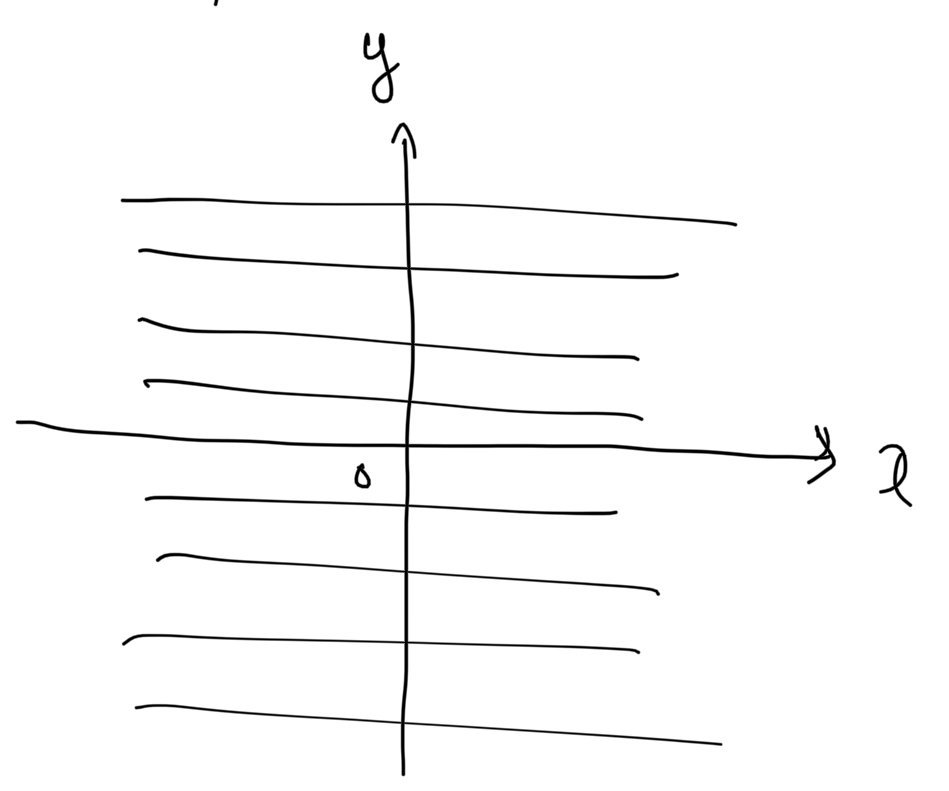
\includegraphics[width=0.7\hsize]{fig1.png}
    \caption{流れ関数$\psi_1$に対応する流れ場の流線}
  \end{minipage}
  \begin{minipage}[b]{0.5\hsize}
    \centering
    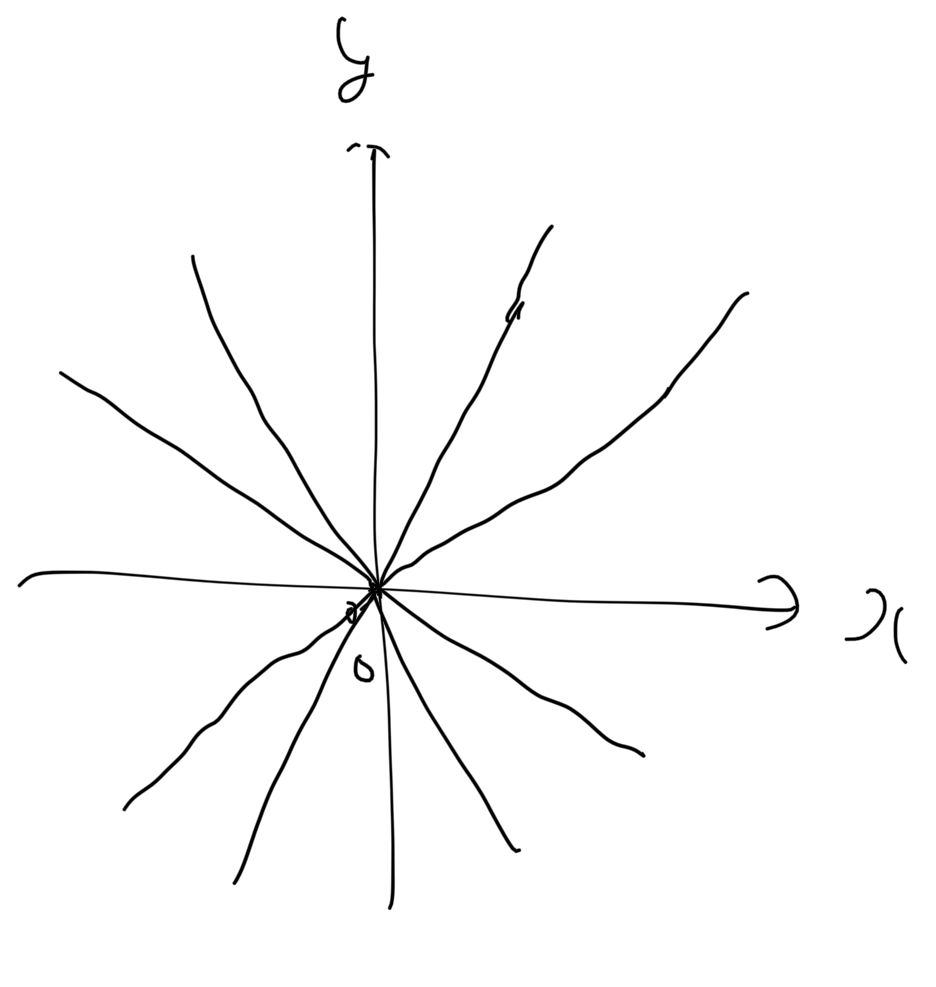
\includegraphics[width=0.7\hsize]{fig2.png}
    \caption{流れ関数$\psi_2$に対応する流れ場の流線}
  \end{minipage}
\end{figure}

\subsubsection{}
流速場は速度ポテンシャルの勾配として得られる。よって、
\begin{align}
  \begin{pmatrix}
    u_1 \\ v_1
  \end{pmatrix} &=
  \begin{pmatrix}
    \frac{\partial \phi_1}{\partial x} \\
    \frac{\partial \phi_1}{\partial y}
  \end{pmatrix} =
  \begin{pmatrix}
    V \\ 0
  \end{pmatrix} \\
  \begin{pmatrix}
    u_2 \\ v_2
  \end{pmatrix} &=
  \begin{pmatrix}
    \frac{\partial \phi_2}{\partial x} \\
    \frac{\partial \phi_2}{\partial y}
  \end{pmatrix} =
  \frac{Q}{2 \pi r^2}
  \begin{pmatrix}
    x \\ y
  \end{pmatrix} \\
  \begin{pmatrix}
    u_3 \\ v_3
  \end{pmatrix} &=
  \begin{pmatrix}
    \frac{\partial \phi_3}{\partial x} \\
    \frac{\partial \phi_3}{\partial y}
  \end{pmatrix} =
  \begin{pmatrix}
    \frac{\partial \phi_1}{\partial x} \\
    \frac{\partial \phi_1}{\partial y}
  \end{pmatrix} +
  \begin{pmatrix}
    \frac{\partial \phi_2}{\partial x} \\
    \frac{\partial \phi_2}{\partial y}
  \end{pmatrix} =
  \begin{pmatrix}
    V + \frac{Q x}{2 \pi r^2} \\
    \frac{Q y}{2 \pi r^2}
  \end{pmatrix}
\end{align}
となる。

\subsubsection{}
Eulerの運動方程式
\begin{equation}
  \frac{\partial \bm{u}}{\partial t} + \left(\bm{u} \cdot \bm{\nabla}\right) \bm{u}
  = -\frac{\bm{\nabla} p}{\rho} + \bm{f}
\end{equation}
において、定常性より$\frac{\partial \bm{u}}{\partial t} = \bm{0}$、
およびベクトル解析の公式
\begin{equation}
  \left(\bm{u} \cdot \bm{\nabla}\right) \bm{u} = \frac{1}{2} \bm{\nabla} (\bm{u} \cdot \bm{u}) - \bm{u} \times (\bm{\nabla \times \bm{u}})
\end{equation}
を代入すると、
\begin{equation}
  \frac{\bm{\nabla} p}{\rho} + \frac{1}{2} \bm{\nabla} (\bm{u} \cdot \bm{u}) - \bm{f}
  = \bm{u} \times (\bm{\nabla \times \bm{u}})
\end{equation}
を得る。ここで、渦なし流れを仮定し$\bm{\nabla \times \bm{u}} = \bm{0}$として、$xy$平面内で物体力がなく
$\bm{f} = \bm{0}$とすると、
\begin{equation}
  \bm{\nabla} \left(\frac{p}{\rho g} + \frac{1}{2g}\left|\bm{u}\right|^2\right) = \bm{0}
\end{equation}
を得る。

\subsubsection{}
式(31)を点Aと点Bを結ぶ任意の経路で線積分すると、
\begin{equation}
  \int_{A \rightarrow B} \bm{\nabla} \left(\frac{p}{\rho g} + \frac{1}{2g}\left|\bm{u}\right|^2\right) \cdot \mathrm{d} \bm{r} = 
  \frac{\Delta p}{\rho g} + \frac{1}{2g} \left(\left|\bm{u}_B\right|^2 - \left|\bm{u}_A\right|^2\right)
  =\bm{0}
\end{equation}
となるため、
\begin{equation}
  \Delta p = -\frac{1}{2} \rho \left(\left|\bm{u}_B\right|^2 - \left|\bm{u}_A\right|^2\right)
\end{equation}
である。これより、
$\Delta p_1 = 0, \Delta p_2 = -\frac{3 \rho Q^2}{8 \pi^2}, \Delta p_3 = -\frac{1}{2} \rho \left(\frac{2 V Q}{\pi} + \frac{3 Q^2}{4 \pi^2}\right)$となる。 

\subsubsection{}
$\bm{u}_3 = \bm{u}_1 + \bm{u}_2$であるが、$\Delta p_3 \neq \Delta p_1 + \Delta p_2$となっている。
Bernoulliの定理に非線形項$\frac{1}{2}\left|\bm{u}\right|^2$があるため、線形的な足し合わせとして扱うことができない。

\subsection{}
\subsubsection{}
流速は速度ポテンシャルの勾配として得られる。
\begin{align}
  u = \frac{\partial \phi}{\partial x}
  = \frac{g a k}{\omega} \frac{\cosh k (z + h)}{\cosh kh} \cos (k x - \omega t) \\
  w = \frac{\partial \phi}{\partial z}
  = \frac{g a k}{\omega} \frac{\sinh k (z + h)}{\cosh kh} \sin (k x - \omega t)
\end{align}
となる。

\subsubsection{}
式(28),(29)より、
\begin{equation}
  \frac{\partial \bm{u}}{\partial t} + \frac{\bm{\nabla} p}{\rho} + \frac{1}{2} \bm{\nabla} (\bm{u} \cdot \bm{u}) - \bm{f}
  = \bm{u} \times (\bm{\nabla \times \bm{u}})
\end{equation}
を得る。
$\bm{u} = \bm{\nabla} \phi, \bm{u} \cdot \bm{u} = u^2 + w^2, f = -\bm{\nabla} (g z), \bm{\nabla} \times \bm{u} = \bm{0}$
を代入すると、
\begin{equation}
  \bm{\nabla} \left(\frac{1}{g} \frac{\partial \phi}{\partial t} + 
  \frac{p}{\rho g} + \frac{1}{2g}\left(u^2 + w^2\right) + z\right) = \bm{0}
\end{equation}
を得る。

\subsubsection{}
式[4]を$t$で微分すると、
\begin{equation}
\frac{\partial \phi}{\partial t} = -g a \frac{\cosh k(z + h)}{\cosh kh} \cos (kx - \omega t)
\end{equation}
水底面での圧力を$p$とする。
式(37)を水底面から水面までの任意の経路$C$で線積分し、$u^2 \simeq w^2 \simeq 0$とすると、
\begin{equation}
  \int_C \bm{\nabla} \left(\frac{1}{g} \frac{\partial \phi}{\partial t} + 
  \frac{p}{\rho g} + \frac{1}{2g}\left(u^2 + w^2\right) + z\right) \cdot \mathrm{d} \bm{r}
  = \frac{1}{g} \left(\left.\frac{\partial \phi}{\partial t}\right|_{z = \eta} - \left.\frac{\partial \phi}{\partial t}\right|_{z = -h}\right)
  + \frac{p_0 - p}{\rho g} + \{\eta - (-h)\} = 0
\end{equation}
となる。ここで、式[5]と式(38)を用いると、
\begin{equation}
  p = p_0 + \rho g h + \frac{\rho g \eta}{\cosh k h}
\end{equation}
を得る。

\subsubsection{}
式(40)において、時間変化する成分は$\rho g \eta / \cosh k h$であり、静水圧は
\begin{equation}
  p - \frac{\rho g \eta}{\cosh k h} = p_0 + \rho g h
\end{equation}
である。\par
この静水圧は時間変化しないが、(c)で求めた圧力は時間変化する。\par
深海波では$\rho g \eta / \cosh k h \simeq \rho g \eta e^{-k h}$であり、動圧の大きさが急激に小さくなる。
圧力変動が信号のノイズに埋もれないよう高精度の計測を行う必要がある。
\end{document}
